%% 
%% Copyright 2019-2020 Elsevier Ltd
%% 
%% This file is part of the 'CAS Bundle'.
%% --------------------------------------
%% 
%% It may be distributed under the conditions of the LaTeX Project Public
%% License, either version 1.2 of this license or (at your option) any
%% later version.  The latest version of this license is in
%%    http://www.latex-project.org/lppl.txt
%% and version 1.2 or later is part of all distributions of LaTeX
%% version 1999/12/01 or later.
%% 
%% The list of all files belonging to the 'CAS Bundle' is
%% given in the file `manifest.txt'.
%% 
%% Template article for cas-sc documentclass for 
%% double column output.

%\documentclass[a4paper,fleqn,longmktitle]{cas-sc}
\documentclass[a4paper,fleqn]{cas-sc}
\usepackage{graphicx}
\usepackage{caption}
\usepackage{subcaption}

% \usepackage[numbers]{natbib}
%\usepackage[authoryear]{natbib}
\usepackage[authoryear,longnamesfirst]{natbib}

%%%Author definitions
\def\tsc#1{\csdef{#1}{\textsc{\lowercase{#1}}\xspace}}
\tsc{WGM}
\tsc{QE}
\tsc{EP}
\tsc{PMS}
\tsc{BEC}
\tsc{DE}
%%%

% Uncomment and use as if needed
%\newtheorem{theorem}{Theorem}
%\newtheorem{lemma}[theorem]{Lemma}
%\newdefinition{rmk}{Remark}
%\newproof{pf}{Proof}
%\newproof{pot}{Proof of Theorem \ref{thm}}

\begin{document}
\let\WriteBookmarks\relax
\def\floatpagepagefraction{1}
\def\textpagefraction{.001}

% Short title
\shorttitle{Reflective Centralities}

% Short author
\shortauthors{O. Lizardo}

% Main title of the paper
\title [mode = title]{Reflective Centralities}                      
% Title footnote mark
% eg: \tnotemark[1]
\tnotemark[1]

% Title footnote 1.
% eg: \tnotetext[1]{Title footnote text}
% \tnotetext[<tnote number>]{<tnote text>} 
\tnotetext[1]{Work on this paper was partially supported by National Science Foundation grant \#.}

%\tnotetext[2]{The second title footnote which is a longer text matter
   %to fill through the whole text width and overflow into
   %another line in the footnotes area of the first page.}


% First author
%
% Options: Use if required
% eg: \author[1,3]{Author Name}[type=editor,
%       style=chinese,
%       auid=000,
%       bioid=1,
%       prefix=Sir,
%       orcid=0000-0000-0000-0000,
%       facebook=<facebook id>,
%       twitter=<twitter id>,
%       linkedin=<linkedin id>,
%       gplus=<gplus id>]
\author[1]{Omar Lizardo}[orcid=0000-0002-5405-3007]

% Corresponding author indication
\cormark[1]

% Footnote of the first author
%\fnmark[1]

% Email id of the first author
\ead{olizardo@soc.ucla.edu}

% URL of the first author
\ead[url]{https://olizardo.github.io/mysite/}

%  Credit authorship
\credit{Conceptualization of this study, Methodology, Software}

% Address/affiliation
\affiliation[1]{organization={University of California, Los Angeles},
    addressline={375 Portola Plaza, 264 Haines Hall}, 
    city={Los Angeles},
    % citysep={}, % Uncomment if no comma needed between city and postcode
    postcode={90095}, 
    state={CA},
    country={U.S.A}}
% Corresponding author text
\cortext[cor1]{Corresponding author}
%\cortext[cor2]{Principal corresponding author}

% Footnote text
%\fntext[fn1]{This is the first author footnote}
%\fntext[fn2]{Another author footnote}

% For a title note without a number/mark
%\nonumnote{This note has no numbers.}

% Here goes the abstract
\begin{abstract}
This template helps you to create a properly formatted \LaTeX\ manuscript.

\noindent\texttt{\textbackslash begin{abstract}} \dots 
\texttt{\textbackslash end{abstract}} and
\verb+\begin{keyword}+ \verb+...+ \verb+\end{keyword}+ 
which
contain the abstract and keywords respectively. 

\noindent Each keyword shall be separated by a \verb+\sep+ command.
\end{abstract}

% Use if graphical abstract is present
% \begin{graphicalabstract}
% \includegraphics{figs/grabs.pdf}
% \end{graphicalabstract}

% Research highlights
\begin{highlights}
\item Research highlights item 1
\item Research highlights item 2
\item Research highlights item 3
\end{highlights}

% Keywords
% Each keyword is seperated by \sep
\begin{keywords}
Centrality \sep Eigenvector \sep Two-Mode Networks \sep Reflective
\end{keywords}


\maketitle

\section{Introduction}
This paper aims to conceptually unify various node centrality measures for one and two-mode networks proposed in the literature under the general idea of \textit{reflective centrality} \citep{hidalgo_hausmann09}. In sociology, due to the great influence of the work of \citet{bonacich72, bonacich87, bonacich91, bonacich_lloyd01}, these types of centralities are usually classified under the general heading of ``eigenvector'' centrality. This is because most of these measures are equivalent to calculating the leading eigenvector of some (possible transformation of the) affinity matrix between nodes, most typically the adjacency matrix (or affiliation matrix for two-mode networks), using standard linear algebra methods. 

My main argument is that the focus on jumping straight to the ``eigenvector'' type status of these measures---essentially a black box linear algebra operation---is misleading in a couple of respects. First, it obscures the underlying \textit{model} of the underlying network process implied by the measure, which is the main claim that a given mathematical operation on the affinity matrix returns something worth calling a ``centrality'' measure \citep{borgatti05}. This is usually a model of the social mechanism that explains why centrality should be ``reflective'' in the first place---e.g., maybe because networks are seen as reflective ``prisms'' indicative of the idea of ``you are the company you keep'' rather than pipes that transmit some kind of good \citep{podolny96}. This underlying social model is more transparently revealed by returning to its ``reflective'' status as given by a set of iterative procedures that result in the ranking of the nodes (in two-mode networks, this involves iterations across the two node sets). 

Secondly, a focus on the iterative process that underlies the measures shows that their eigenvector status is mathematically derivative and not crucial to their status as social network measures of centrality. This is because iteration happens to be a method for computing the leading eigenvector of a matrix satisfying a set of (generally weak) properties---the so-called ``power method.'' The reflective iteration is crucial from a social science perspective since this reveals the underlying \textit{assumptions} made by the model as to how the social mechanism alluded to earlier works on a relational basis. 

Recasting these measures as reflective iterations makes these assumptions explicit, thus potentially helping us choose between different variants of different reflective centralities depending on their fit to our favorite theory. As we will see later, a focus on reflection can also help us better see the commonalities across many variations of these ``eigenvector-style'' measures, some proposed outside social network analysis proper, including fields like information science. 

In sum, unifying eigenvector-style measures by focusing on their reflective status can thus help us bring conceptual clarity to this largely disorganized field, laying bare some of the core assumptions behind the social exchange, prestige, or status model implicit in their construction. It can also help us develop a more abstract ``schema'' for what a general reflective centrality metric should look like. This schema can then be used to develop novel reflective centrality measures by plugging in proximity or similarity matrices different from those typically used in previous work or motivated by alternative models of the social mechanism, explaining how direct and indirect connections can acquire reflective properties.  

The rest of the paper is organized as follows \ldots

\begin{figure}[h!t!]
    \captionsetup[subfigure]{font=footnotesize,labelfont=footnotesize}
     \centering
     \begin{subfigure}[b]{0.45\textwidth}
        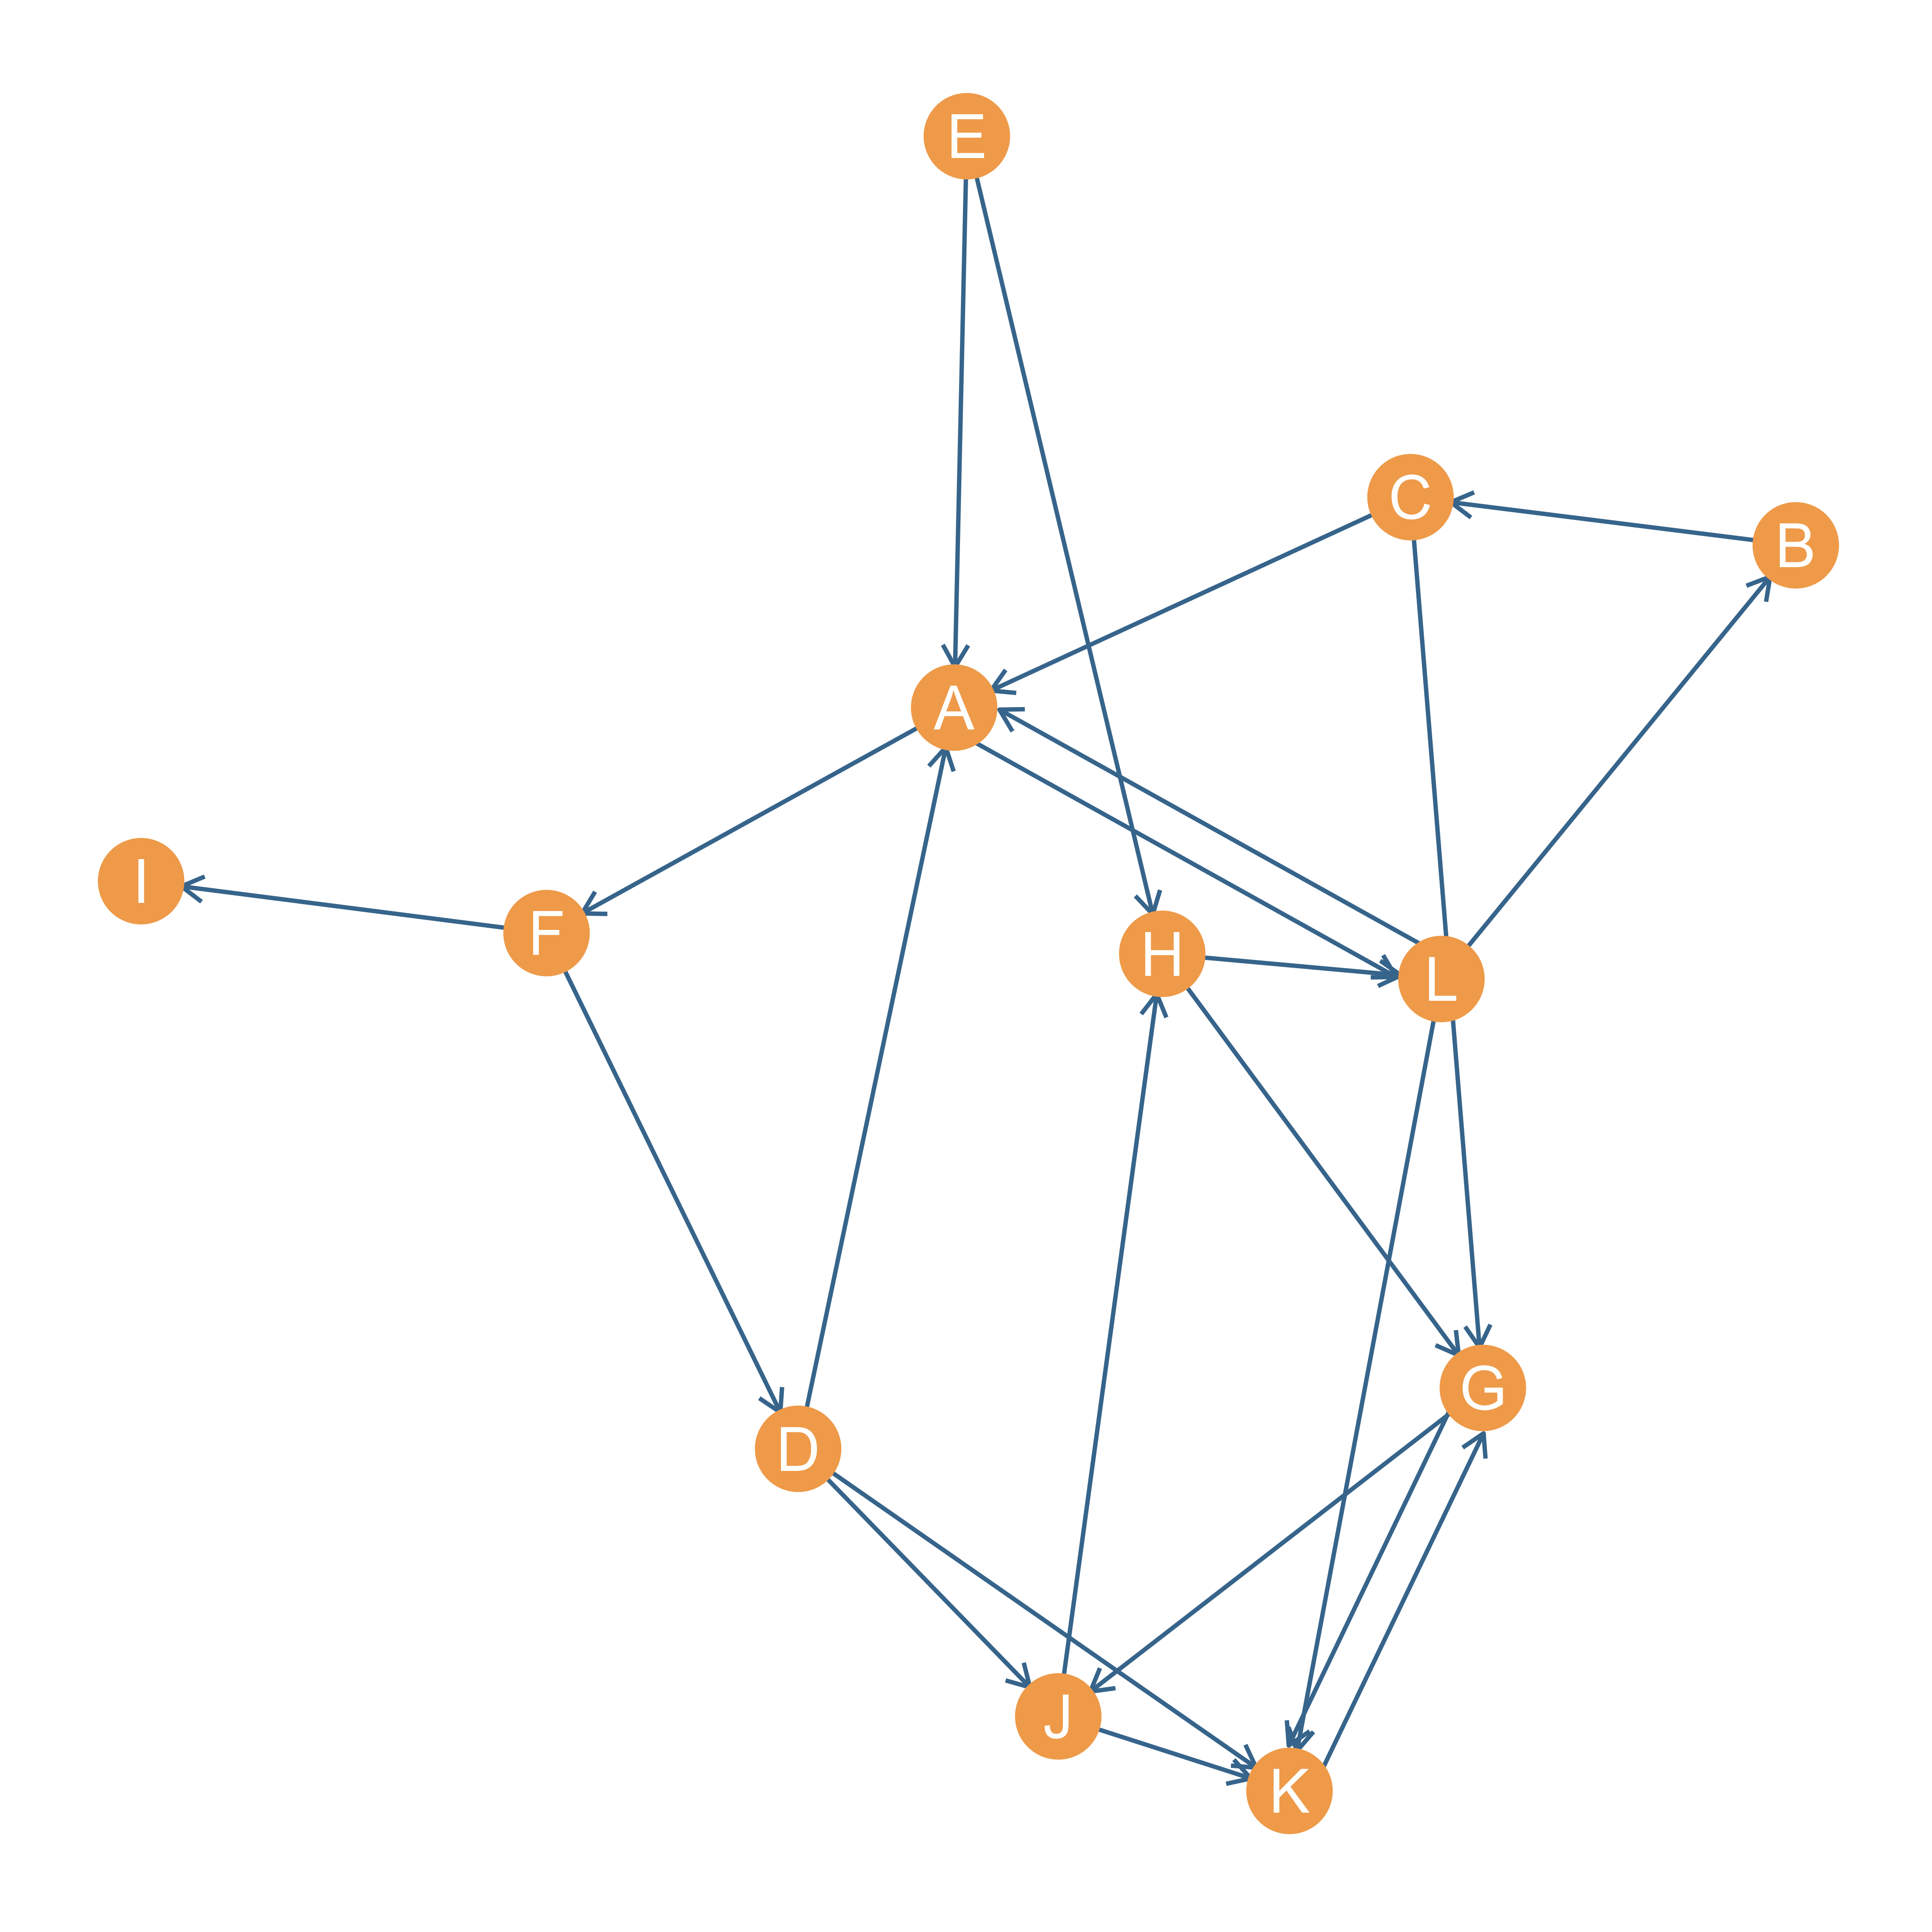
\includegraphics[width=1.0\textwidth]{Plots/directed.png}
        \caption{}
        \label{fig:directed}
    \end{subfigure} 
     \begin{subfigure}[b]{0.45\textwidth}
        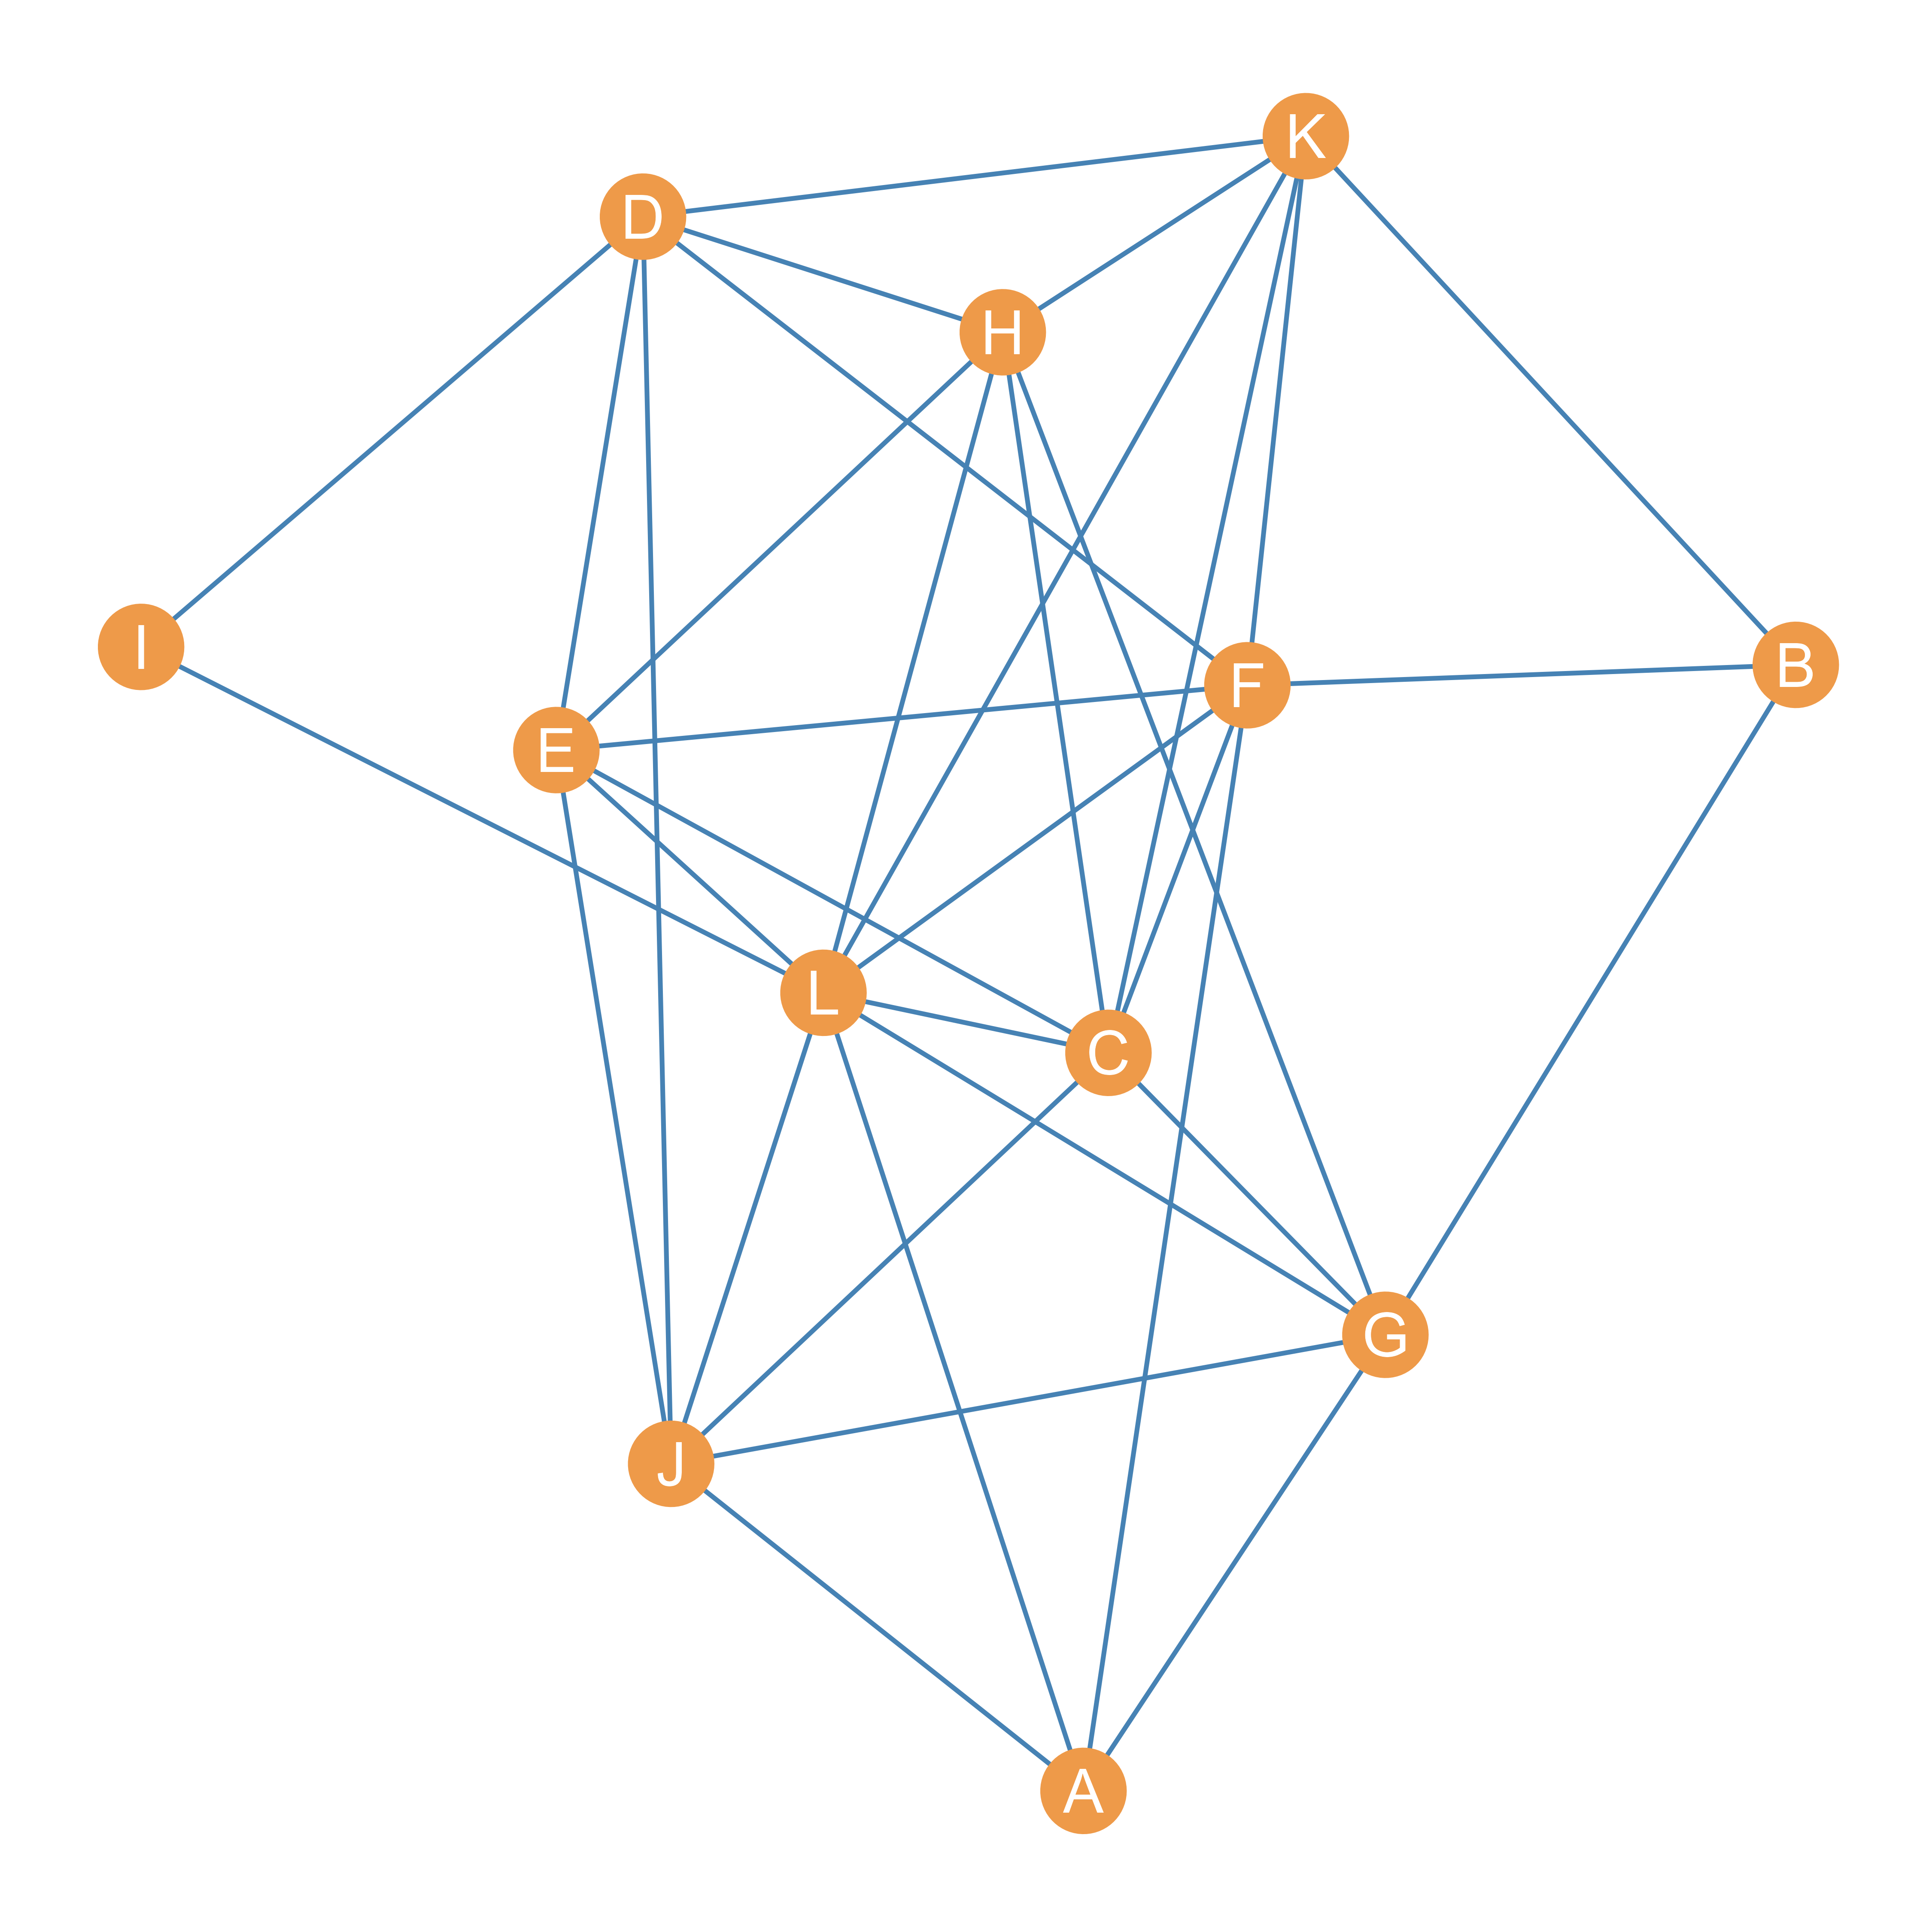
\includegraphics[width=1.0\textwidth]{Plots/undirected.png}
        \caption{}
        \label{fig:undirected}
    \end{subfigure}
\end{figure}

\section{One-Mode Reflective Centralities}
\subsection{Eigenvector Centrality as a Reflective Centrality}
First, I begin with a quick and dirty criterion for counting a given centrality measure as ``reflective.'' A measure of centrality is reflective if the centrality of a given node is a function of the centrality of other nodes in the graph, usually nodes that are adjacent or proximate in some way, and where the centrality of all the nodes is computed on some kind of common scale. 

This definition sets up a classic chicken-or-the-egg problem---or more precisely an ``infinite regress'' \citep[234-235]{seeley49}---since, to figure out the centrality of a node, we need to know the centrality of the other nodes in the graph it is linked to, but to know the centrality of these other nodes, we need to know the centrality of the others \textit{they} are connected to and so forth. 

Although usually not presented in this way, given the straight jump to computing eigenvectors, the classic Bonacich eigenvector centrality is ``reflective'' in this sense since for any node $i$ connected to some other set of nodes $i$, their centrality is given by:

\begin{equation}
    x_i = \sum_j a_{ij}x_j
    \label{eq:bon1}
\end{equation}

In matrix form:

\begin{equation}
    \mathbf{x} = \mathbf{A} \mathbf{x}
    \label{eq:bon2}
\end{equation}

This means that a simple reflective algorithm to compute the $\mathbf{x}$ vector is simply to initialize the vector $\mathbf{x}$ at step $q = 0$ with some uniform set of positive values---let us say the unit vector $\mathbf{1}$ of the same length as the number of nodes in the graph. We can then use~\ref{eq:bon1} to compute the centralities of the nodes at each step according to:

\begin{equation}
    \mathbf{x}(q) = \mathbf{A} \mathbf{x}(q - 1)
    \label{eq:bon3}
\end{equation}

And after this is done for each step $q > 0$:

\begin{equation}
    \mathbf{x}(q) = \frac{\mathbf{x}(q)}{||\mathbf{x}(q)||_2}
    \label{eq:bon4}
\end{equation}

Where the denominator in~\ref{eq:bon4} is the Euclidean vector norm.\footnote{For any vector $\mathbf{x}$ of length $n$, the $L_2$ norm is: $||\mathbf{x}||_2 = \sqrt{\sum_i^n x_i^2}$. Dividing by any vector norm---e.g., the $L_1$ or max norm---will prevent divergence and return scores perfectly correlated to the leading eigenvector approach. Dividing by the $L_2$ norm returns scores that are \textit{exactly} the same, save for rounding error, as the absolute value of the dominant right eigenvector of the adjacency matrix.} As we progress in the series of iterations $q = \{1, 2, 3, \ldots\}$, $\mathbf{x}$ is bound to converge (as long as we apply the normalization) to a steady value. These values will be equivalent (up to rounding error) to the (absolute value) of the dominant right eigenvector of $\mathbf{A}$.

But this eigenvector property is less revealing regarding the type of centrality computed by~\ref{eq:bon2} than a focus on the iterative reflective process itself, even though this iteration is seldom made apparent in presentations of the eigenvector centrality. What is revealed here is the set of assumptions implicit in the standard Bonacich centrality. These can be glossed as follows: (1) At each step, each node in the graph receives the same amount of (normalized) centrality from each of its neighbors, implying that (2) nodes distribute the same ``amount'' to each of their neighbors regardless of their own level of connectivity. This gives the centrality of each node at $q$. At $q + 1$, each node repeats that step with the centrality they accumulated in the previous round, and so on, until convergence.  The ``top'' (most central) nodes are the ones bound to receive the most \textit{total} normalized centrality from their neighbors---who received it from their neighbors, who received it from their neighbors---as $q$ approaches a limit. 

\begin{table}[!h]
\centering
\centering
\begin{tabular}[t]{>{}lr}
\toprule
\textbf{I} & 0.406\\
\textbf{B} & 0.384\\
\textbf{L} & 0.362\\
\textbf{K} & 0.352\\
\textbf{J} & 0.294\\
\textbf{F} & 0.282\\
\textbf{H} & 0.282\\
\textbf{D} & 0.236\\
\textbf{E} & 0.236\\
\textbf{C} & 0.173\\
\textbf{G} & 0.160\\
\textbf{A} & 0.143\\
\bottomrule
\end{tabular}
\centering
\begin{tabular}[t]{lr}
\toprule
\textbf{L} & 0.585\\
\textbf{I} & 0.481\\
\textbf{K} & 0.353\\
\textbf{G} & 0.286\\
\textbf{B} & 0.272\\
\textbf{F} & 0.228\\
\textbf{J} & 0.223\\
\textbf{A} & 0.155\\
\textbf{C} & 0.088\\
\textbf{H} & 0.088\\
\textbf{E} & 0.068\\
\textbf{D} & 0.000\\
\bottomrule
\end{tabular}
\end{table}


\subsection{The Seeley/PageRank Index as a Reflective Centrality}
The assumptions encoded in the classic Bonacich reflective centrality are reasonable but not the only ones we can make. Changing the assumptions leads to a different reflective measure. For instance, take assumption (2) above. This assumption could be questioned. Perhaps a more sensible assumption is that nodes do not distribute the same quantum of centrality to their neighbors regardless of their own degree. Instead, each node ``gets'' some centrality from their neighbor that is \textit{proportional} to their neighbor's degree, with neighbors taking the same centrality quantum, dividing it according to how many neighbors they have, and then sending it along. Thus, a node with many neighbors distributes less centrality to each one of its neighbors than a node with just a few neighbors.

How would we modify~\ref{eq:bon3} to reflect this model of the social process? Consider the matrix $\mathbf{P}$ defined as:

\begin{equation}
    \mathbf{P} = \mathbf{D}^{-1} \mathbf{A}
\end{equation}

Where $\mathbf{D}$ is a matrix with each node's (out)degrees along the diagonals and zeroes in every other cell. The matrix $\mathbf{P}$ is row stochastic, and its entries are equivalent to the original adjacency matrix with each cell divided by the row total (equivalent to applying the $L_1$ norm to the vectors formed by the rows of the $\mathbf{A}$ the matrix). Substantively, each cell entry in $\mathbf{P}$ equals the \textit{probability} that a random walker that starts in node $i$ ends up in $j$ for node pairs $i,j$ in the graph. The matrix $\mathbf{P}$ thus defines a Markov chain on the graph, with each state of the Markov chain at $t$ equal to the node the random walker is at time $t$ and each cell entry defining the conditional probability that the walker will end up at a given node $j$ at $t$ given that it was at another node $i$ at $t-1$.

To calculate the corresponding reflective centrality, we can just plug $\mathbf{P}$ instead of $\mathbf{A}$ into a slightly modified version of equation~\ref{eq:bon3} to get the following:

\begin{equation}
    \mathbf{x}(q) = \mathbf{P}^T \mathbf{x}(q - 1)
    \label{eq:seeley1}
\end{equation}

With $\mathbf{x}(0) = \mathbf{1}$ and $\mathbf{P}^T$ being the tranpose of $\mathbf{P}$. Like~\ref{eq:bon3}, the vector $\mathbf{x}$ in~\ref{eq:seeley1} converges to the leading eigenvector of $\mathbf{P}^T$. But more important is the reflective interpretation: At each step $q$, each node's centrality is the sum of the contributions made by their in-neighbors, which are weighted by their degree. Getting a nomination from someone who gives out nominations like candy counts for less in making you central than being tapped by someone who is more selective. 

The rank order of nodes computed by~\ref{eq:seeley1} is equivalent to a long-lost reflective centrality index proposed by \citet{seeley49} and discussed by \citet{vigna16}, but more popularly known recently as the---simple, with dampening factor $\alpha$ set to 1.0---version of the PageRank centrality index \citep{brinn_page}. 

As \citet[218]{fouss_etal16} note, this reflective centrality admits to two interpretations. One more properly reflective (networks as prisms) says that~\ref{eq:seeley1} calculates a ``global endorsement score quantifying the overall support'' nodes in the graph receive from others. The other one, more consistent with a ``networks as pipes'' model, says that~\ref{eq:seeley1} calculates the stationary probability of finding a random walker at any given node for each node in the graph. 

Either interpretation shows that this is an entirely different model of the underlying social process than that suggested by equation~\ref{eq:bon3}, so the best way to think of it is as a modified version of the usual Bonacich reflective centrality with the modification reflecting (pun intended) a different model of how centrality is reflectively distributed in the social system \citep{seeley49}.

\subsection{Kleinberg's Hubs and Authorities Score as a Reflective Centrality}
So far, we have considered reflective centralities that work directly with the adjacency matrix or some modification thereof but compute a single reflective centrality at a time. However, in many cases, centralities are not only \textit{reflective}, they may also be \textit{reflexive}; that is, two kinds of reflective centralities are defined in terms of one another. In one-mode networks, this is the most likely case for directed relations, where the meaning of incoming links differs from those of outgoing links. 

One reflective centrality for which a strong ``reflexive'' argument has been made is Kleinberg's \citeyearpar{kleinberg99} hubs and authorities index. One interesting aspect of this measure is that it was proposed from the get-go as a reflective centrality with a transparent iterative algorithm (with proof that the algorithms converged to the eigenvector of a matrix) that also makes transparent its reflexive nature. 

The basic idea behind Kleinberg's ``HITS'' measure---with the acronym standing for ``Hyperlink-Induced Topic Search,'' reflecting its origins in information science---is that in any directed network where the reflective currency is some kind of ``endorsement'' relative to the authority of a given object or person (e.g., as in a who-goes-to-whom for advice network), an ``authoritative'' node receives endorsement, not just from any old person, but from ``discerning'' others.  ``Discerning'' others, in turn, are those people who specialize in endorsing authoritative nodes. 

This creates a classic snake-eating-its-own-tail problem with two types of ``simultaneous'' reflective centralities defined reflexively. As we will see later, eight years before Kleinberg, \citet{bonacich91} had proposed a similar approach to calculating ``simultaneous'' reflective-reflexive centralities for the two sets of nodes in two-mode networks, although without necessarily making their reflective status completely transparent. As we will also see later, making this status transparent helps us better see the links between the Bonacich approach and other reflective centralities proposed for two-mode networks. 

In any case, in the one-mode case, we can solve the infinite regress problem of figuring out who an authority and a discerning ``hub'' (in Kleinberg's terminology) is. We simply define each in terms of the other:

\begin{equation}
    \begin{split}
    &\mathbf{x}_a = \sum_j a_{ij} \mathbf{x}_h \\
    &\mathbf{x}_h = \sum_i  a_{ij} \mathbf{x}_a 
    \end{split}
    \label{eq:klein1}
\end{equation}

Equation~\ref{eq:klein1} just says that the authority score $\mathbf{x}_a$ of a given node is just the sum of the hub scores $\mathbf{x}_h$ of the nodes that point to it. Authorities are people endorsed by discerning others. Who's discerning? According to~\ref{eq:klein1}, your discerning abilities $\mathbf{x}_h$ are just the sum of the authoritativeness $\mathbf{x}_a$ of the people you endorse. To algorithmically compute the required $\mathbf{x}_a$ and $\mathbf{x}_h$ scores references inn~\ref{eq:klein1}, we just initialize the vector $\mathbf{x}_h(0)$ to a set of positive constant values of length $n$ equal to $\frac{1}{\sqrt{{n}}}$ (where $n$ is the number of nodes) and compute the following iteration until both scores converge:

\begin{equation}
    \begin{split}
        &\mathbf{x}_a(q) = \mathbf{A}^T\mathbf{x}_h(q-1) \\
        &\mathbf{x}_h(q) = \mathbf{A}\mathbf{x}_a(q) \\
    \end{split}
    \label{eq:klein2}
\end{equation}

While making sure to normalize both $\mathbf{x}_a(q)$ and $\mathbf{x}_h(q)$ by the Euclidean---or some other---vector norm at each step $q > 0$ before feeding them to the next equation. The reflective process depicted in equation~\ref{eq:klein2} effectively says that a node's authority score is just the sum of the hub scores of its in-neighbors. In contrast, a node's hub score is just the sum of the authority scores of its out-neighbors, as reflectively calculated in the previous step. This measure, therefore, captures the ``doubling'' of reflective centralities in the directed case, where people\ get centrality from being pointed to by central others. Central others get their centrality by pointing to central people, thus ``mutually reinforcing'' \citep[136]{lempel_moran01} each other's authority and hub status. 

Just like the other reflective centralities considered, Kleinberg shows that the final $\mathbf{x}_a$ and $\mathbf{x}_h$ vectors end up being the solutions to a leading eigenvector problem (thus qualifying this centrality as part of the family of eigenvector centralities). Specifically, the convergent $\mathbf{x}_a$ score is the leading eigenvector of the common in-neighbors matrix $\mathbf{A}^T\mathbf{A}$. The $\mathbf{x}_h$ score is the leading eigenvector of the common out-neighbors matrix $\mathbf{A}\mathbf{A}^T$. Alternatively, $\mathbf{x}_a$ and $\mathbf{x}_h$ are the left and right singular vectors of the adjacency matrix $\mathbf{A}$, respectively.

\subsection{SALSA as a Reflective Centrality}
We can imagine combining the reflective approach behind the Seeley/PageRank reflective centrality index and Kleinberg's Hubs and Authorities approach, as was done by \citet{lempel_moran01} when they developed their SALSA---``Stochastic Approach for Link Structure Analysis''---algorithm as a variant of Kleinberg's approach. As before, this involves modifying the underlying model of how centrality is reflected in the system and defined reflexively. 

What underlying assumptions can we modify? Like the Bonacich centrality, Kleinberg's HITS algorithm presumes that hubs and authorities receive the \textit{same} ``amount'' of centrality points from their out and in-neighbors (respectively) regardless of their hub and authority status (e.g., their out and in-degree). \citet{lempel_moran01} use the same reasoning that led us to question this assumption in the Bonacich centrality case---which led us to the PageRank/Seeley reflective centrality---to modify Kleinberg's HITS as follows.

%At each step, we assume that each authority distributes some ``amount' of centrality to each hub that points to them \textit{relative} to that authority's in-degree, such that authorities that are pointed to by many other nodes count for less. The hub score of each node is then the sum of this quantity across all their out-neighbors (potential authorities). At the same time, we also assume that each hub distributes some ``amount'' of centrality to the hubs that point to them relative to their out-degree, such that hubs that point to many other authorities are discounted compared to more selective hubs. The authority score of each node is then the sum of this quantity across all their out-neighbors (potential authorities). Here, the reflective-reflexive centrality is conceptualized as a \textit{dissipative} quantity that gets smaller if extended too far in either direction. These diminishing returns are then reflexively projected to the corresponding hub and authorities scores.

At the initial step, each node begins with authority and hub vectors equal to uniform positive values of the same length as the number of nodes in the graph normalized so that their sum of squares is equal to unity: $\mathbf{x}(0)_h = \mathbf{x}(0)_a = \frac{1}{\sqrt{n}}$, where $n$ is the number of nodes. We also define a new matrix $\mathbf{W}=\mathbf{C}^{-1} \mathbf{A}$, with $\mathbf{C}$ being a diagonal matrix containing the column sums of $\mathbf{A}$---each node's in-degree---as its diagonal entries and zeroes in every other cell. We can then iteratively calculate the authority and hub scores of each node using the following equation:

\begin{equation}
    \begin{split}
        &\mathbf{x}_a(q) = \mathbf{W}^T\mathbf{x}_h(q-1) \\
        &\mathbf{x}_h(q) = \mathbf{P}\mathbf{x}_a(q-1) \\
        &(q > 0)
    \end{split}
    \label{eq:salsa}
\end{equation}

Equation~\ref{eq:klein2} differs from~\ref{eq:salsa} only in terms of (1) the matrices that we plug into the reflective steps \citep{lempel_moran01}, substituting  $\mathbf{W}^T$ for $\mathbf{A}^T$ and $\mathbf{P}$ for $\mathbf{A}$ respectively, and (2) initializing both hub and authority scores at the outset, while using the previous versions of each until convergence \citep[1186]{farahat_etal06}. 

Like the Kleinberg HITS index, the convergent SALSA reflective centralities are identical to the absolute value of the leading eigenvector of a matrix. In the case of $\mathbf{x}_a$ this is the matrix $\mathbf{W}^T\mathbf{P} = \left(\mathbf{C}^{-1}\mathbf{A}\right)^T\mathbf{D}^{-1}\mathbf{A}$, while for $\mathbf{x}_h$ this is the matrix $\mathbf{P}\mathbf{W}^T = \mathbf{D}^{-1}\mathbf{A}\left(\mathbf{C}^{-1}\mathbf{A}\right)^T$.

The reflective interpretation of~\ref{eq:salsa} goes as follows: at each step the authority scores of each node are the sum of the hub scores of each of the nodes that point to it, as in~\ref{eq:klein2}, but this time, a hub counts for more in a node's authority score \textit{the less} other nodes point to it (as given by the in-degree weight in $\mathbf{W}$). The measure thus emphasizes ``pure'' hubs in constructing a node's authority score, people who point to others but are not pointed to by many others. A hub's authority score is reflexively built the same way as the sum of the authority scores of the nodes it points to, except that potential authority nodes that point to many other nodes are discounted as authorities in constructing a node's hub score (as given by the out-degree weight in $\mathbf{P}$), thus giving preference to ``pure'' authorities (nodes that are pointed to by many others but don't point to others). 

\subsection{CA as a Reflective Centrality}
Correspondence Analysis (CA) has been advocated for before in social network analysis as a method to analyze square adjacency matrices \citep{noma_smith85}, with an emphasis on finding ``optimal scores'' to re-arrange the rows and columns of the matrix to reveal a grouping pattern (in the style of blockmodeling). In this section, I show that, in addition to doing that, the scores corresponding to the first dimension of a simple CA of the adjacency matrix can also be interpreted as a type of reflective centrality for directed graphs based on \textit{averages} (of averages) of the in(out) degrees of the nodes that a given node sends(receives) ties to(from). In essence, the reflective centrality model underlying CA of the adjacency matrix can be considered a modification of the process exemplified by the SALSA approach in~\ref{eq:salsa}, where we indeed move from sums to averages.

At each step, we assume that each hub distributes some ``amount' of centrality to each authority they point to relative to their own out-degree. The authority score of each node is then the average of this quantity across all their in-neighbors (potential hubs). At the same time, we also assume that each authority distributes some ``amount'' of centrality to the hubs that point to them relative to their own in-degree. The hub score of each node is then the average of this quantity across all their out-neighbors (potential authorities). At the initial step, each node begins with authority and hub scores equal to their in and out-degree.  

In reflective terms:

\begin{equation}
    \begin{split}
        &\mathbf{x}_a(q) = \frac{\mathbf{A}^T\mathbf{x}_h(q-1)}{\mathbf{x}_a(0)}  \\
        &\mathbf{x}_h(q) = \frac{\mathbf{A}\mathbf{x}_a(q)}{\mathbf{x}_h(0)}  \\ 
        & (q > 0) \\ \\
        &\mathbf{x}_a(0) = k^{in} = \sum_i a_{i.} \\
        &\mathbf{x}_h(0) = k^{out} = \sum_j a_{.j}     
    \end{split}
    \label{eq:ca1}
\end{equation}

Where $k^{in}$ is just the vector of node in-degrees, and $k^{out}$ is the vector of out-degrees. At step $q = 1$, equation~\ref{eq:ca1} says that the authority score of each node ($\mathbf{x}_a(1)$) is just the sum of the outdegrees ($\mathbf{x}_h(0)$) of the nodes that point to them averaged across all their in-neighbors ($\mathbf{x}_a(0)$). The hub score of each node at the same time step is just this last quantity ($\mathbf{x}_a(1)$) averaged across all their out-neighbors ($\mathbf{x}_h(0)$). We then iterate until there is negligible change in authority and hub scores between iterations. Because we are taking averages of sums of averages of sums of averages, the differences between authority and hub scores across nodes will decrease toward zero as we iterate. We can keep the respective scores spread apart using the usual z-score normalization at each step before feeding it forward:

\begin{equation}
    \begin{split}
        &\mathbf{x}_a(q) = \frac{\mathbf{x}_a(q) - \mathbf{\Bar{x}}_a(q)}{sd(\mathbf{x}_a(q))} \\
        &\mathbf{x}_h(q) = \frac{\mathbf{x}_h(q) - \mathbf{\Bar{x}}_h(q)}{sd(\mathbf{x}_h(q))} \\ 
        & (q > 0) 
    \end{split}
    \label{eq:ca-norm}
\end{equation}

Where $\mathbf{\Bar{x}}(q)$ is the mean of the authority or hub score vector, and $sd(\mathbf{x}(q))$ is the standard deviation of the same vector. What do these scores converge toward? It turns out that as we iterate across steps, we end up coming up with a vector perfectly correlated to the subdominant eigenvector (corresponding to the second largest eigenvalue) of the matrix $(\mathbf{D}_{i}^{-1} \mathbf{A}^T \mathbf{D}_{o}^{-1} \mathbf{A})$ (for the authority scores) and the matrix $(\mathbf{D}_{o}^{-1} \mathbf{A} \mathbf{D}_{i}^{-1} \mathbf{A}^T)$ (for the hub scores), where $\mathbf{D}_{i}$ is the diagonal matrix containing the $k^{in}$ vector along the diagonals and $\mathbf{D}_{o}$ is the corresponding diagonal out-degree matrix (for both these matrices the dominant eigenvector, corresponding to $\lambda_1 = 1$ is the ``trivial'' vector containing constant entries). Note these matrices are essentially the common in and out-neighbor matrices---which are the matrices whose eigenvectors the standard Kleinberg reflective centralities converge to---but with the adjacency matrix and its transpose pre-multiplied by the inverse of the out and in-neighbors of each node before being multiplied by one another. Essentially, this involves moving from raw sums in the Kleinberg approach to averages.

Importantly, it has been shown that the reflective centrality computed in equation~\ref{eq:ca1} is equivalent to the row and column scores for the correspondence analysis of the original adjacency matrix. 


%% Loading bibliography style file
% \bibliographystyle{model1-num-names}
\bibliographystyle{cas-model2-names}

% Loading bibliography database
\bibliography{cas-refs}


\end{document}


The Elsevier cas-sc class is based on the
standard article class and supports almost all of the functionality of
that class. In addition, it features commands and options to format the
\begin{itemize} \item document style \item baselineskip \item front
matter \item keywords and MSC codes \item theorems, definitions and
proofs \item lables of enumerations \item citation style and labeling.
\end{itemize}

This class depends on the following packages
for its proper functioning:

\begin{enumerate}
\itemsep=0pt
\item {natbib.sty} for citation processing;
\item {geometry.sty} for margin settings;
\item {fleqn.clo} for left aligned equations;
\item {graphicx.sty} for graphics inclusion;
\item {hyperref.sty} optional packages if hyperlinking is
  required in the document;
\end{enumerate}  

All the above packages are part of any
standard \LaTeX{} installation.
Therefore, the users need not be
bothered about downloading any extra packages.

\section{Installation}

The package is available at author resources page at Elsevier
(\url{http://www.elsevier.com/locate/latex}).
The class may be moved or copied to a place, usually,\linebreak
\verb+$TEXMF/tex/latex/elsevier/+, %$%%%%%%%%%%%%%%%%%%%%%%%%%%%%
or a folder which will be read                   
by \LaTeX{} during document compilation.  The \TeX{} file
database needs updation after moving/copying class file.  Usually,
we use commands like \verb+mktexlsr+ or \verb+texhash+ depending
upon the distribution and operating system.

\section{Front matter}

The author names and affiliations could be formatted in two ways:
\begin{enumerate}[(1)]
\item Group the authors per affiliation.
\item Use footnotes to indicate the affiliations.
\end{enumerate}
See the front matter of this document for examples. 
You are recommended to conform your choice to the journal you 
are submitting to.

\section{Bibliography styles}

There are various bibliography styles available. You can select the
style of your choice in the preamble of this document. These styles are
Elsevier styles based on standard styles like Harvard and Vancouver.
Please use Bib\TeX\ to generate your bibliography and include DOIs
whenever available.

Here are two sample references: \cite{Fortunato2010}
\cite{Fortunato2010,NewmanGirvan2004}
\cite{Fortunato2010,Vehlowetal2013}

\section{Floats}
{Figures} may be included using the command,\linebreak 
\verb+\includegraphics+ in
combination with or without its several options to further control
graphic. \verb+\includegraphics+ is provided by {graphic[s,x].sty}
which is part of any standard \LaTeX{} distribution.
{graphicx.sty} is loaded by default. \LaTeX{} accepts figures in
the postscript format while pdf\LaTeX{} accepts {*.pdf},
{*.mps} (metapost), {*.jpg} and {*.png} formats. 
pdf\LaTeX{} does not accept graphic files in the postscript format. 

\begin{figure}
	\centering
		\includegraphics[scale=.75]{figs/Fig1.pdf}
	\caption{The evanescent light - $1S$ quadrupole coupling
	($g_{1,l}$) scaled to the bulk exciton-photon coupling
	($g_{1,2}$). The size parameter $kr_{0}$ is denoted as $x$ and
	the \PMS is placed directly on the cuprous oxide sample ($\delta
	r=0$, See also Table \protect\ref{tbl1}).}
	\label{FIG:1}
\end{figure}


The \verb+table+ environment is handy for marking up tabular
material. If users want to use {multirow.sty},
{array.sty}, etc., to fine control/enhance the tables, they
are welcome to load any package of their choice and
{cas-sc.cls} will work in combination with all loaded
packages.

\begin{table}[width=.9\linewidth,cols=4,pos=h]
\caption{This is a test caption. This is a test caption. This is a test
caption. This is a test caption.}\label{tbl1}
\begin{tabular*}{\tblwidth}{@{} LLLL@{} }
\toprule
Col 1 & Col 2 & Col 3 & Col4\\
\midrule
12345 & 12345 & 123 & 12345 \\
12345 & 12345 & 123 & 12345 \\
12345 & 12345 & 123 & 12345 \\
12345 & 12345 & 123 & 12345 \\
12345 & 12345 & 123 & 12345 \\
\bottomrule
\end{tabular*}
\end{table}

\section[Theorem and ...]{Theorem and theorem like environments}

{cas-sc.cls} provides a few shortcuts to format theorems and
theorem-like environments with ease. In all commands the options that
are used with the \verb+\newtheorem+ command will work exactly in the same
manner. {cas-sc.cls} provides three commands to format theorem or
theorem-like environments: 

\begin{verbatim}
 \newtheorem{theorem}{Theorem}
 \newtheorem{lemma}[theorem]{Lemma}
 \newdefinition{rmk}{Remark}
 \newproof{pf}{Proof}
 \newproof{pot}{Proof of Theorem \ref{thm2}}
\end{verbatim}


The \verb+\newtheorem+ command formats a
theorem in \LaTeX's default style with italicized font, bold font
for theorem heading and theorem number at the right hand side of the
theorem heading.  It also optionally accepts an argument which
will be printed as an extra heading in parentheses. 

\begin{verbatim}
  \begin{theorem} 
   For system (8), consensus can be achieved with 
   $\|T_{\omega z}$ ...
     \begin{eqnarray}\label{10}
     ....
     \end{eqnarray}
  \end{theorem}
\end{verbatim}  


\newtheorem{theorem}{Theorem}

\begin{theorem}
For system (8), consensus can be achieved with 
$\|T_{\omega z}$ ...
\begin{eqnarray}\label{10}
....
\end{eqnarray}
\end{theorem}

The \verb+\newdefinition+ command is the same in
all respects as its \verb+\newtheorem+ counterpart except that
the font shape is roman instead of italic.  Both
\verb+\newdefinition+ and \verb+\newtheorem+ commands
automatically define counters for the environments defined.

The \verb+\newproof+ command defines proof environments with
upright font shape.  No counters are defined. 


\section[Enumerated ...]{Enumerated and Itemized Lists}
{cas-sc.cls} provides an extended list processing macros
which makes the usage a bit more user friendly than the default
\LaTeX{} list macros.   With an optional argument to the
\verb+\begin{enumerate}+ command, you can change the list counter
type and its attributes.

\begin{verbatim}
 \begin{enumerate}[1.]
 \item The enumerate environment starts with an optional
   argument `1.', so that the item counter will be suffixed
   by a period.
 \item You can use `a)' for alphabetical counter and '(i)' 
  for roman counter.
  \begin{enumerate}[a)]
    \item Another level of list with alphabetical counter.
    \item One more item before we start another.
    \item One more item before we start another.
    \item One more item before we start another.
    \item One more item before we start another.
\end{verbatim}

Further, the enhanced list environment allows one to prefix a
string like `step' to all the item numbers.  

\begin{verbatim}
 \begin{enumerate}[Step 1.]
  \item This is the first step of the example list.
  \item Obviously this is the second step.
  \item The final step to wind up this example.
 \end{enumerate}
\end{verbatim}

\section{Cross-references}
In electronic publications, articles may be internally
hyperlinked. Hyperlinks are generated from proper
cross-references in the article.  For example, the words
\textcolor{black!80}{Fig.~1} will never be more than simple text,
whereas the proper cross-reference \verb+\ref{tiger}+ may be
turned into a hyperlink to the figure itself:
\textcolor{blue}{Fig.~1}.  In the same way,
the words \textcolor{blue}{Ref.~[1]} will fail to turn into a
hyperlink; the proper cross-reference is \verb+\cite{Knuth96}+.
Cross-referencing is possible in \LaTeX{} for sections,
subsections, formulae, figures, tables, and literature
references.

\section{Bibliography}

Two bibliographic style files (\verb+*.bst+) are provided ---
{model1-num-names.bst} and {model2-names.bst} --- the first one can be
used for the numbered scheme. This can also be used for the numbered
with new options of {natbib.sty}. The second one is for the author year
scheme. When  you use model2-names.bst, the citation commands will be
like \verb+\citep+,  \verb+\citet+, \verb+\citealt+ etc. However when
you use model1-num-names.bst, you may use only \verb+\cite+ command.

\verb+thebibliography+ environment.  Each reference is a\linebreak
\verb+\bibitem+ and each \verb+\bibitem+ is identified by a label,
by which it can be cited in the text:

\noindent In connection with cross-referencing and
possible future hyperlinking it is not a good idea to collect
more that one literature item in one \verb+\bibitem+.  The
so-called Harvard or author-year style of referencing is enabled
by the \LaTeX{} package {natbib}. With this package the
literature can be cited as follows:

\begin{enumerate}[\textbullet]
\item Parenthetical: \verb+\citep{WB96}+ produces (Wettig \& Brown, 1996).
\item Textual: \verb+\citet{ESG96}+ produces Elson et al. (1996).
\item An affix and part of a reference:\break
\verb+\citep[e.g.][Ch. 2]{Gea97}+ produces (e.g. Governato et
al., 1997, Ch. 2).
\end{enumerate}

In the numbered scheme of citation, \verb+\cite{<label>}+ is used,
since \verb+\citep+ or \verb+\citet+ has no relevance in the numbered
scheme.  {natbib} package is loaded by {cas-sc} with
\verb+numbers+ as default option.  You can change this to author-year
or harvard scheme by adding option \verb+authoryear+ in the class
loading command.  If you want to use more options of the {natbib}
package, you can do so with the \verb+\biboptions+ command.  For
details of various options of the {natbib} package, please take a
look at the {natbib} documentation, which is part of any standard
\LaTeX{} installation.

\appendix
\section{My Appendix}
Appendix sections are coded under \verb+\appendix+.

\verb+\printcredits+ command is used after appendix sections to list 
author credit taxonomy contribution roles tagged using \verb+\credit+ 
in frontmatter.

\printcredits




%\vskip3pt

\bio{}
Author biography without author photo.
Author biography. Author biography. Author biography.
Author biography. Author biography. Author biography.
Author biography. Author biography. Author biography.
Author biography. Author biography. Author biography.
Author biography. Author biography. Author biography.
Author biography. Author biography. Author biography.
Author biography. Author biography. Author biography.
Author biography. Author biography. Author biography.
Author biography. Author biography. Author biography.
\endbio

\bio{figs/pic1}
Author biography with author photo.
Author biography. Author biography. Author biography.
Author biography. Author biography. Author biography.
Author biography. Author biography. Author biography.
Author biography. Author biography. Author biography.
Author biography. Author biography. Author biography.
Author biography. Author biography. Author biography.
Author biography. Author biography. Author biography.
Author biography. Author biography. Author biography.
Author biography. Author biography. Author biography.
\endbio

\bio{figs/pic1}
Author biography with author photo.
Author biography. Author biography. Author biography.
Author biography. Author biography. Author biography.
Author biography. Author biography. Author biography.
Author biography. Author biography. Author biography.
\endbio


